\documentclass[12pt,prb,aps,epsf]{article}
\usepackage[utf8]{inputenc}
\usepackage{amsmath}
\usepackage{amsfonts}
\usepackage{amssymb}
\usepackage{graphicx} 
\usepackage{latexsym} 
\usepackage[toc,page]{appendix}
%\usepackage{listings}
\usepackage{xcolor}
\usepackage{soul}
\usepackage[T1]{fontenc}
\usepackage{amsthm}
\usepackage{mathtools}
\usepackage{setspace}
\usepackage{array,multirow,makecell}
\usepackage{geometry}
\usepackage{textcomp}
\usepackage{float}
\usepackage{cancel}
\usepackage{here}
\usepackage{titlesec}
\usepackage{bbold}

\geometry{hmargin=2cm,vmargin=2cm}

\begin{document}
	
	\title{MP 33 Régimes transitoires}
	\author{Maria}
	\date{Agrégation 2019}
	
	\maketitle
	
	\tableofcontents
	
	\pagebreak
	
\subsection{Introduction}
Définir la notion de régime transitoire : passage d'un régime établi à un autre.

\section{Circuit du premier ordre : RC}
On alimente un RC avec un créneau de période $T\geq 5\tau$ où $\tau = RC$. On regarde alors les tensions $U_C$ et $U_R$ à l'oscilloscope pour différentes valeurs de R et de C : R = 10 k$\Omega$, 5 k$\Omega$ et 2 k$\Omega$ (on doit avoir $R_{gene}\ll R \ll R_{oscillo}$ pour qu'un modèle de Rc sans considérer le générateur et l'oscillo convienne), et C = 10 nF, 100 nF et 1$\mu$F. On fait ainsi varier $\tau$ sur une plage de 20 $\mu$s  à 10 ms. Pour chaque combinaison on mesure le temps caractéristique $\tau$, que l'on peut comparer avec l'expression attendue $\tau =RC$ en traçant 
\begin{equation}
\log \tau_{exp} = f(\log \tau_{modele})
\end{equation}
(en log-log pour rentre compte du fait qu'on a 3 ordres de grandeur de temps) et en modélisant par une droite. On peut ensuite vérifier que le coefficient directeur est compatible avec 1, et l'ordonnée à l'origine avec 0.\\

Pour faire office de résidus on peut tracer le rapport $\frac{\tau_{exp}}{\tau_{modele}}$ en fonction du numéro (arbitraire) de la combinaison associée. On voit alors que pour le plus petit $\tau$ il faudrait prendre en compte l'incertitude due à la résistance du générateur $\simeq 1\%$ et peut être la capacité due aux fils (sans doute autour de 1\% aussi).\\

Pour donner du sens à cette manip on peut montrer au préalable qu'on a bien un comportement exponentiel en traçant le logarithme d'une tension acquise sur Latis pro. On démontre ainsi que l'on a un circuit du premier ordre.\\
On constate que la dissipation contrôle la transition vers un nouvel état du système (condensateur déchargé ou chargé selon).\\

Fluctuation dissipation : c'est la résistance qui amène vers l'équilibre, mais c'est elle qui fait qu'on oscille autour de cet équilibre sans jamais y être puisque la dissipation et les fluctuations ne sont que deux faces d'un même phénomène.

\section{Circuit du second ordre : RLC}
On construit un circuit RLC, et on observe les trois régimes possibles : critique (on converge très vite, et sans osciller, vers le nouvel état d'équilibre), apériodique (équivalent à deux circuits du premier ordre, pas très intéressant ici) et pseudo périodique. On observe un régime ou l'autre selon la résistance choisie. \\

On observera ici le régime pseudo périodique où la tension $U_c(t)$ est une sinusoïde amortie (on excite avec un créneau). On modélise $U_c(t)$ avec un modèle du type 
\begin{eqnarray}
U_c(t) = U_0 + Ae^{-\omega_0\xi t}\cos(\omega t + \phi)
\end{eqnarray}
où $\omega = \omega_0 \sqrt{1-\xi^2}$ et $\tau = \frac{1}{\omega_0 \xi}$.
On peut alors comparer les différents éléments donnés par la régression à ceux attendus par notre modèle en vue des valeurs des composantes du circuit.\\

On peut de même calculer le dépassement $D = e^{-\xi\pi/\sqrt{1-\xi^2}}$ qui caractérise l'amplitude max de la tension pendant le régime transitoire par rapport à la tension asymptotique. \\

Là encore c'est la dissipation (résistance) qui dirige le régime transitoire. Il faut prendre une petite résistance afin d'observer un maximum d'oscillations (d'avoir un "bon" facteur de qualité).\\

Le régime transitoire peut se voir comme un échange périodique d'énergie magnétique (bobine) et électrique (condensateur) entre le condensateur et la bobine, échange atténué au cours du temps à cause du fait qu'il y a une résistance entre la capa et la bobine : dissipation.

\section{Diffusion}
\textbf{Regarder Sextant, et Sommerfield}

\begin{figure}[h]
	\centering 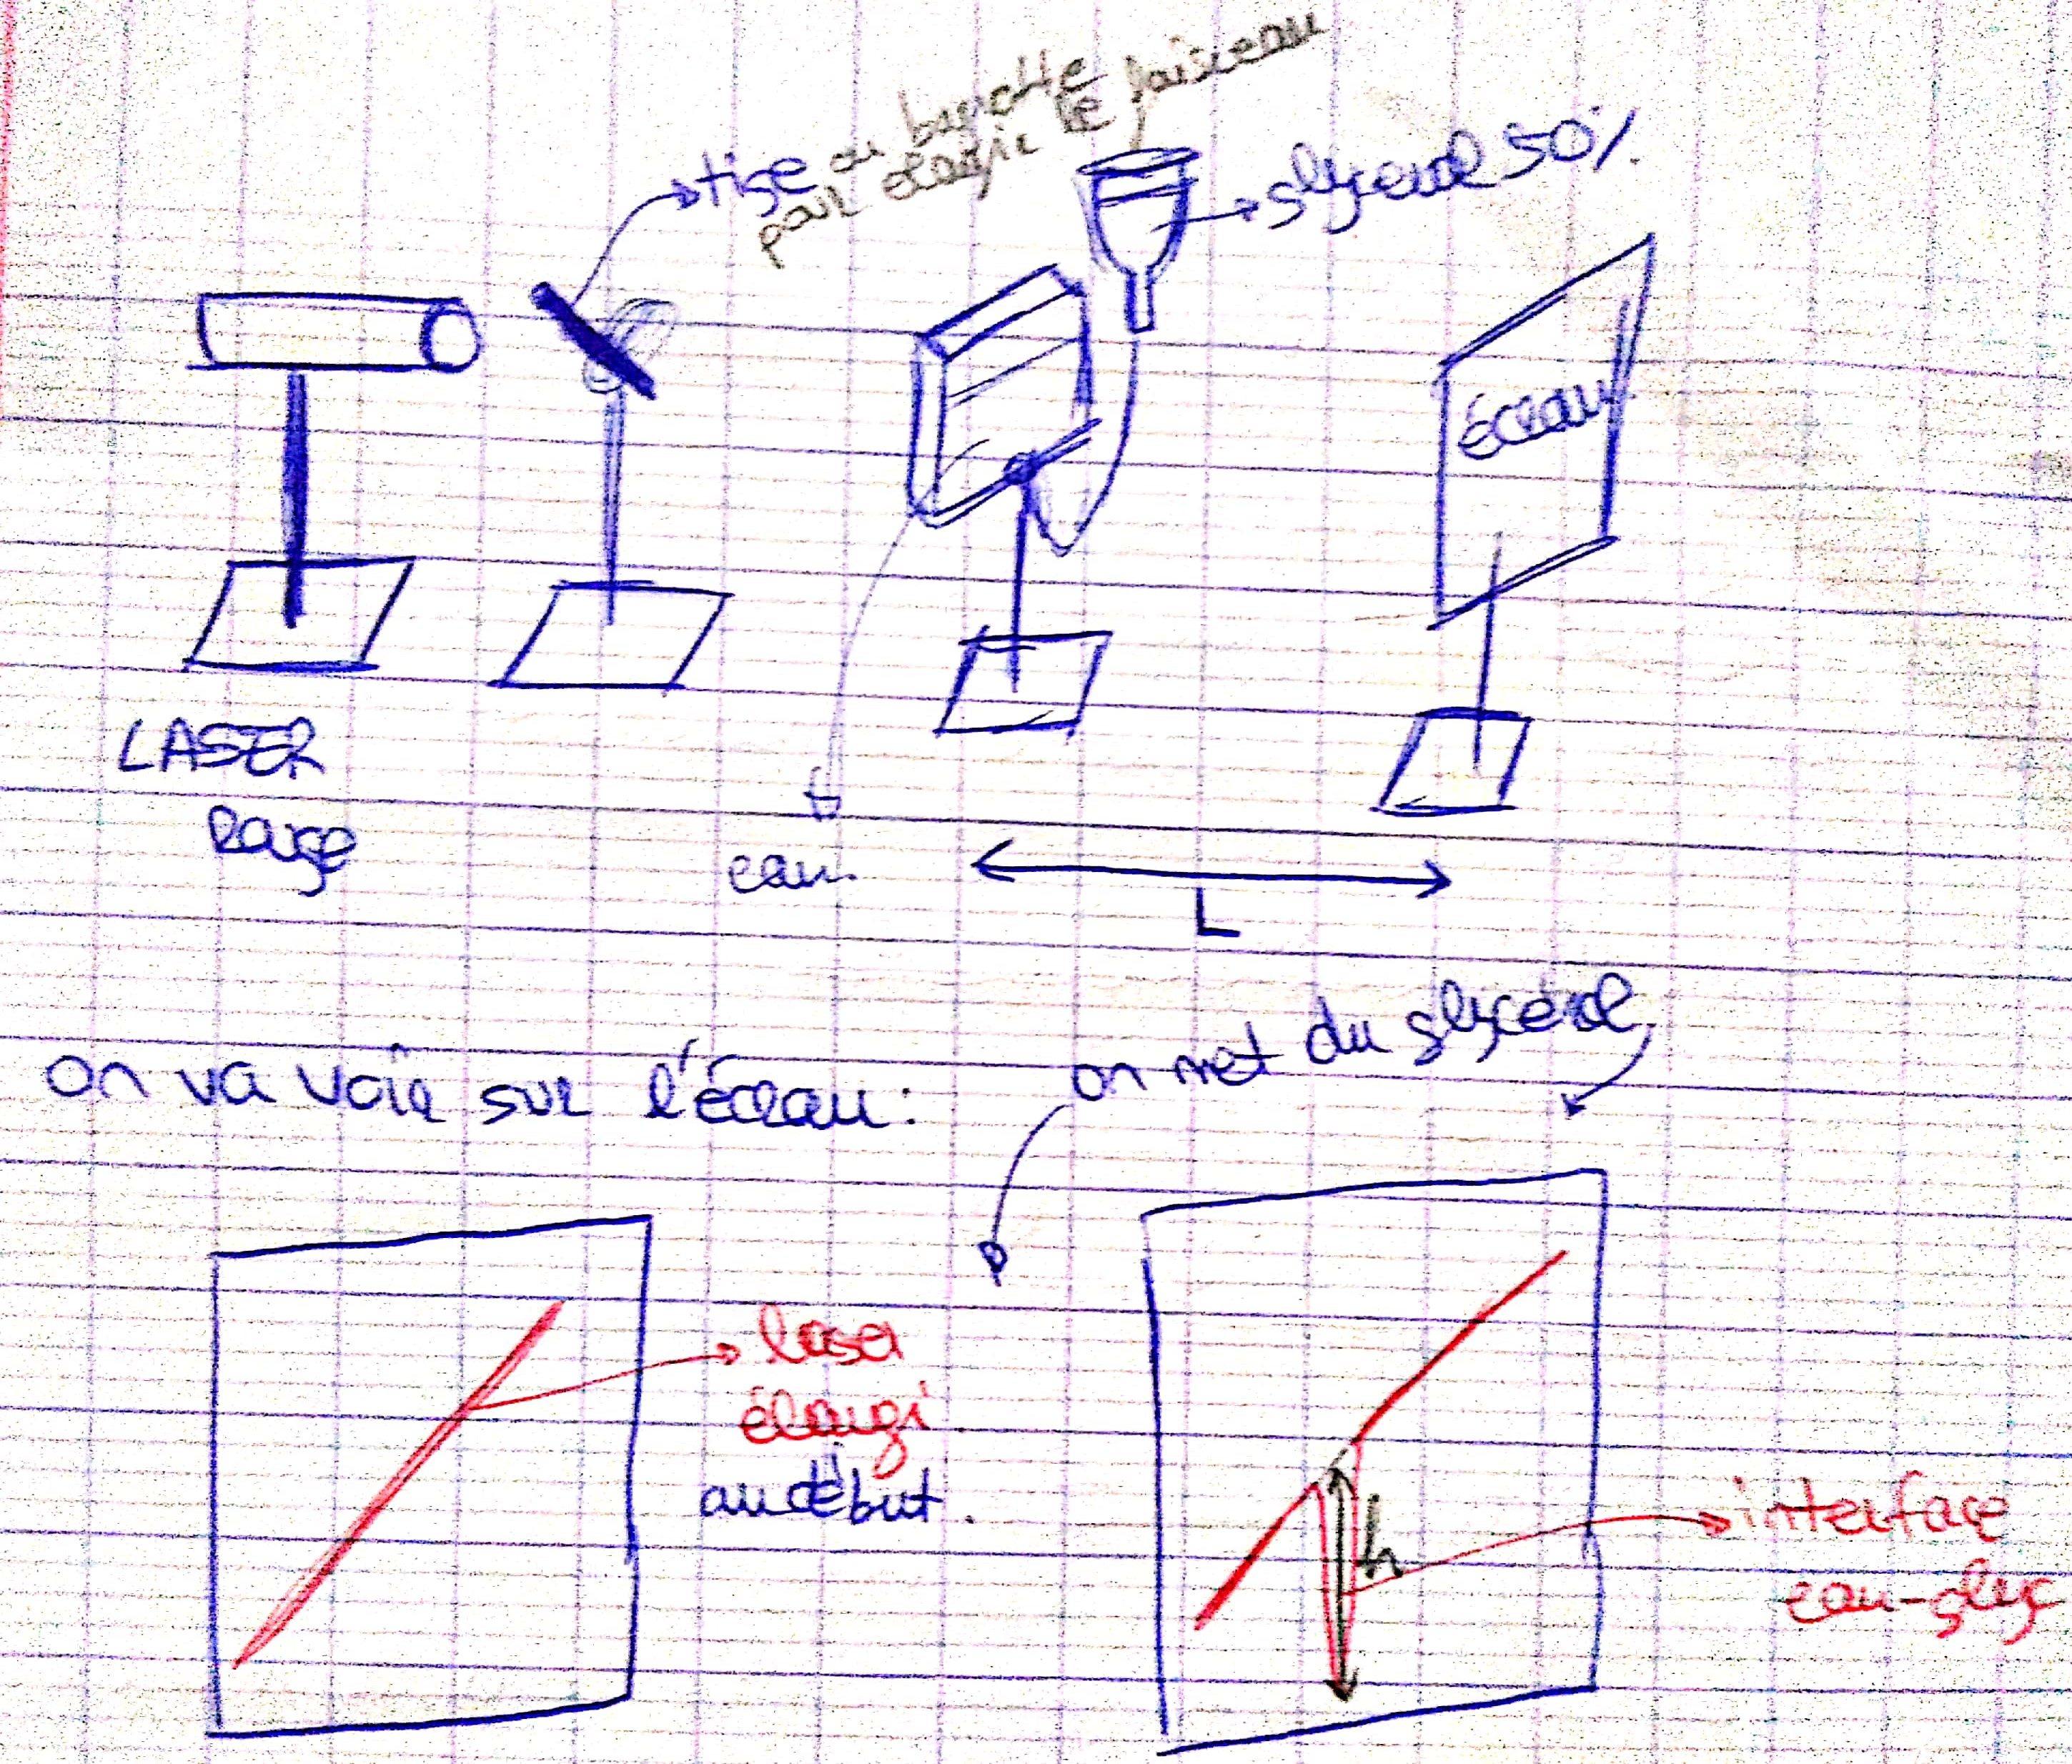
\includegraphics[width=13cm]{schema_diffusion}
\end{figure}
On utilise une cuve avec une interface entre de l'eau et une solution de glycerol à 50\% (on injecte le glycerol en fond de cuve à l'aide d'un tube et d'une seringue). On envoie une nappe de lumière oblique sur la cuve à l'aide d'un laser et d'une baguette de verre. On regarde la figure obtenue par réfraction sur un écran derrière la cuve. On y voit une droite oblique, habillée d'un "pic" en son centre dû au gradient d'indice à l'interface : la hauteur $h$ de ce pic va alors nous permettre de remonter au coefficient de diffusion du glycerol.\\
En combinant équation de diffusion et optique on obtient 
\begin{eqnarray}
\alpha_{max} = \frac{(n_g-n_e)d}{4n_0\sqrt{\ln(2)Dt}}
\end{eqnarray}
avec $\alpha$ l'angle de déviation, L la distance entre l'écran et la cuve, $n_g$ l'indice optique du glycerol et $n_e$ celui de l'eau, $D$ le coefficient de diffusion, et $d$ l'épaisseur de la cuve. On en déduit 
\begin{eqnarray}
\tan \alpha = \frac{h}{L}\;\;\Rightarrow\;\; \frac{1}{\arctan^2{\frac{h}{l}}} = \frac{16n_0^2\ln2\,D}{d^2(n_g-n_e)^2}t
\end{eqnarray}
On va donc mesurer $h$ et tracer $\frac{1}{\arctan^2{\frac{h}{l}}}$ (on étudie de la diffusion : on s'attend à une distance carré qui varie linéairement avec le temps) en fonction du temps, modéliser par une droite. A partir du coefficient directeur de cette droite $a$ on peut alors déduire la valeur du coefficient de diffusion
\begin{eqnarray}
D = \frac{ad^2(n_g-n_e)^2}{16n_0^2\ln2}\hspace{1cm} \frac{u(D)}{D} \simeq \frac{u(a)}{a}
\end{eqnarray}
On pourra ensuite vérifier que $D$ est bien dans l'intervalle attendu 
\begin{eqnarray}
D_{att} \in [1,10].10^{-10}\,\mathrm{m}^3.s^{-1}
\end{eqnarray}

On doit attendre que l'interface se stabilise avant de pouvoir faire la mesure, mais cela signifie qu'au début de la mesure on aura déjà un mélange partiel entre les deux solutions (eau et glycerol).

\paragraph{Conclusion}: Nous avons mis en valeur le caractère déterminant de la dissipation (résistance et viscosité) dans les régimes transitoires.

\section*{Questions}
Qu'est ce que le dépassement ?\\
C'es défini comme $\frac{U_c^{max}-U_0}{U_0}$ avec $U_0$ la tension échelon d'alimentation. Cela caractérise l'amplitude max de la tension pendant le régime transitoire par rapport à la tension asymptotique.\\

Quel est l'intérêt de cette notion ?\\

Quel est l'intérêt de ces régimes ?\\

Pourquoi le régime critique est il souhaitable ?\\
Car dans ce cas la durée du régime transitoire est minimale. Exemple : amortisseur : on ne veut pas que lors d'une secousse l'amortisseur oscille (longtemps).\\

Comment fait on alors pour se placer dans ce régime (quand on est initialement en pseudo périodique)?\\
on augmente le frottement (la résistance)...

\end{document}